\section{Experimentación}

Como ya hemos mencionado, a lo largo de este trabajo practico analizaremos diferentes tipos de estrategias para resolver el problema del CIDM. Para poder comparar entre estrategias, experimentaremos con cada algoritmo utilizando 6 familias de grafos diferentes, las cuales serán descriptas a continuación.

\subsection{Grafos Aleatorios}

Se tomaron grafos aleatorios para poder experimentar con situaciones mas generales, en donde el resultado es usualmente impredecible a simple vista. Los grafos aleatorios son generados en base a dos variables, estas son:

\begin{itemize}
	\item La cantidad de nodos (de aquí en adelante $n$)
	\item La cantidad de conexiones entre nodos (de aquí en adelante $m$)
\end{itemize}

Para la experimentación se decidió variar el $n$ principalmente, sin embargo, también es pertinente investigar el impacto que pueden llegar a tener la cantidad de conexiones en el grafo. Para cada valor de $n$ se generaron 3 grafos con diferentes valores de $m$, estos fueron $\frac{n}{2}$, $n$ y $2n$.

\subsection{Grafos $d$-regulares conexos}

Esta familia fue elegida ya que podemos dar la cantidad de nodos que conforman el CIDM, esta es $\lceil\frac{n}{d}\rceil$ \textbf{FALTA JUSTIFICAR}. Podemos ver esto en el siguiente ejemplo:

\begin{figure}[ht]
\centering
\begin{subfigure}[b]{0.4\textwidth}
	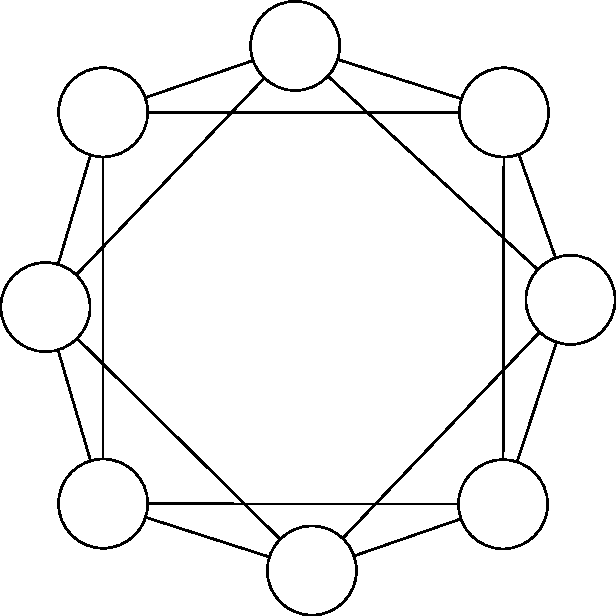
\includegraphics[scale=0.6]{images/dRegular.pdf}
	\caption{$n = 8, d = 4$}
\end{subfigure}
\begin{subfigure}[b]{0.4\textwidth}
	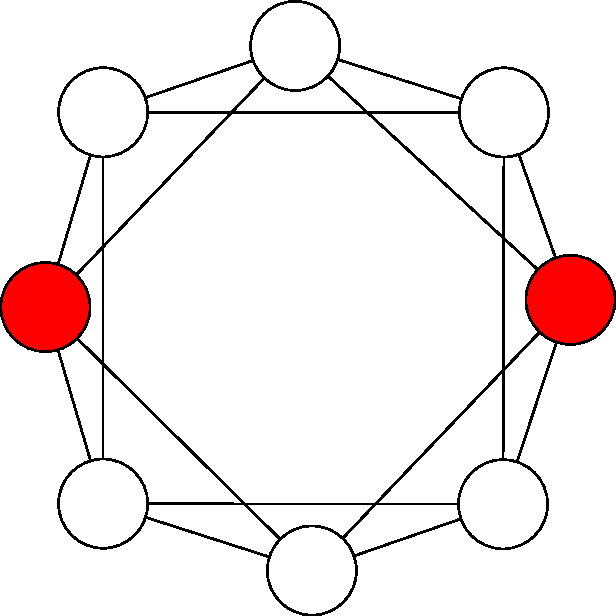
\includegraphics[scale=0.6]{images/dRegularSol.pdf}
	\caption{$\lceil\frac{8}{4}\rceil = 2$}
\end{subfigure}
\end{figure}

Esto nos permite hacer un análisis sobre el tamaño de las soluciones, permitiéndonos tener una mejor perspectiva a la hora de elegir la mejor configuración. Al igual que con los aleatorios, estos grafos poseen dos variable, las cuales son:

\begin{itemize}
	\item La cantidad de nodos
	\item El grado de los nodos (la variable $d$)
\end{itemize}
	
Se siguió una metodología similar que en el caso aleatorio, es decir, para cada $n$ se tomaron 3 valores de $d$, que fueron $\frac{n}{4}$, $\frac{n}{2}$ y $\frac{3n}{4}$.

\subsection{Grafos bipartitos completos}

Al igual que en el caso anterior, la principal razón por la cual decidimos probar con esta familia es que podemos determinar el tamaño de la solución de antemano. Como el grafo es bipartito completo, alcanza con tomar todos los nodos de alguno de los dos conjuntos para poder obtener un CIDM, es decir que para todo grafo bipartito completo la solución va a ser el tamaño del conjunto mas pequeño. Las variables involucradas en este caso son:

\begin{itemize}
	\item La cantidad de nodos en la primer componente
	\item La cantidad de nodos en la segunda componente
\end{itemize}

Para la experimentación se vario la cantidad de nodos de la primer componente, y para cada una de ellas se generaron dos grafos bipartitos completos con $\frac{n}{4}$ y $\frac{3n}{4}$.

\subsection{Arboles binarios}

A diferencia de las dos familias anteriores, donde el tamaño de la solución es único, aquí nos encontramos con un caso donde hay mas de una. Si en un árbol tomamos todos los nodos de un nivel, en el próximo no seria necesario tomar ninguno en el próximo, este patrón se repita hasta llegar al ultimo nivel. Dependiendo de la cantidad de niveles, esto nos permite dar una cota inferior para el CIDM, estas son:

\begin{itemize}
	\item Si la cantidad de niveles es par ($log_2(n)\mod 2 = 0$), la cota inferior es $\mathlarger{\mathlarger{‎\sum}}_{i=0}^{\frac{log_2(n)}{2} - 1} 2^{2i}$
		\item Si la cantidad de niveles es impar ($log_2(n)\mod 2 \neq 0$), la cota inferior es $\mathlarger{\mathlarger{‎\sum}}_{i=0}^{\lfloor\frac{log_2(n)}{2}\rfloor - 1} 2^{2i + 1}$
\end{itemize}

Podemos ver esto en el siguiente ejemplo:

Para todo árbol sabemos que la cantidad de conexiones es igual a la cantidad de nodos menos uno, es por esto que para la experimentación se vario únicamente la cantidad de nodos.

\subsection{Cliques}

Al igual que los casos anteriores, se probo también con cliques ya que para cualquier grafo de esta familia sabemos el tamaño de la solución. Para cualquier clique alcanza con tomar un nodo para poder obtener un CIDM, ya que desde esto nodo puedo alcanzar el resto de los nodos del grafo. La idea detrás de experimentar con esta familia es probar la eficiencia de los algoritmos, ya que los mismos deberían poder resolver estos grafos de manera veloz y eficiente.

Al igual que con los arboles binarios, para generar estos grafos solo entra en juego una única variable, y es la cantidad de nodos en el mismo. Al ser una clique, la cantidad de conexiones es siempre $\frac{n(n-1)}{2}$.

\subsection{Grafos unión de componentes conexas}

Por ultimo se decidió probar con un grafo formado por varias componente conexas, unidas por puentes. Cada una de las componentes conexas es un $C_i$, para generar estos grafos se crean sucesivos $C_i$, tomando inicialmente $i = 1$ y aumentando la cantidad de nodos siempre y cuando la cantidad total de nodos los permita. Una vez que las tenemos generadas, se la comienza a unir de manera sucesiva, es decir, se une $C_1$ con $C_2$, $C_2$ con $C_3$, así hasta llegar al ultimo camino generado. La motivación para probar esta familia es poder analizar el impacto que puede llegar a tener la resolución de cada una de las componentes, teniendo en cuenta la presencia de ejes puentes, los cuales pueden afectar el tiempo que toma resolver el grafo.

Esta familia se reservo para ser utilizada como \texttt{test set} al momento de elegir los parámetros óptimos para GRASP. El resto de las familias las utilizaremos como \texttt{training set}.

\subsection{Metodología}

Para hacer el análisis, se hizo variar el valor de $n$ entre 10 y 220. Si el generador para alguna de las familias recibe un segundo parámetro, los utilizados son los mencionados en la sección de cada familia. Para cada valor de $n$ se corrió el algoritmo 100 veces y se tomo el promedio del tiempo.